\documentclass[titlepage]{article}

\usepackage{float}
\usepackage[T1]{fontenc}
\usepackage[utf8]{inputenc}
\usepackage[english]{babel}
\usepackage{minted}
\usepackage{graphicx}
\usepackage{geometry}
\usepackage{amsmath}
\usepackage{appendix}
\usepackage{comment}
\usepackage{hyperref}
\usepackage{caption}
\usepackage{amssymb}


\geometry{hmargin=3cm,vmargin=2cm}

\usepackage[
backend=biber,
style=alphabetic,
sorting=ynt
]{biblatex}
\addbibresource{ref.bib}

\begin{document}
\begin{titlepage}
\newcommand{\HRule}{\rule{\linewidth}{0.5mm}}
\center
\textsc{\LARGE
Information and Coding Theory 
} \\[1cm]
\textsc{\LARGE
ELEN060-2
} \\[1cm]

\includegraphics[scale=0.2]{logo.jpg} \\[3cm]
\HRule \\[0.4cm]
{ \huge \bfseries Project 1 - Information measures \\[0.15cm] }
\HRule \\[1.5cm]
Destexhe Clara S191103 \\
Hogge Louis S192814
\\[1.5cm]
\today \\ [1cm]
\end{titlepage}


\section{Implementation}

\subsection*{Question 1 : Entropy}

Entropy is a measure of uncertainty in a random variable. It quantifies the amount of information a random variable is expected to contain. It is computed in bits due to the log in base two. The minus is added to counter the logarithm value (always negative). Indeed, entropy is never negative. \\

If $\mathcal{X}$ is a discrete random variable and $P(X_i)$ the value of the probability distribution of the event $\mathcal{X}_i$, then the entropy of $\mathcal{X}$ is :

$$H(\mathcal{X}) \triangleq-\sum_{i=1}^n P\left(\mathcal{X}_i\right) \log_2 P\left(\mathcal{X}_i\right)$$

In order to compute the entropy, a sum is done on the elements of the probability distribution vector. Zero probabilities are not considered in the sum, thanks to the added condition in the loop. 

\subsection*{Question 2 : Joint Entropy}

The joint entropy measures of uncertainty related to a set of random variables. The entropy and the joint entropy have the same formula but the joint probability matrix replaces the probability vector. The matrix is a 2-D array; thus, a sum is added to consider each element in the formula. \\

If $\mathcal{X}$ and $\mathcal{Y}$ are discrete random variables, $P\left(\mathcal{X}_i \cap \mathcal{Y}_j\right)$ is the probability of the random variable $\mathcal{X}$ to be $\mathcal{X}_i$ and in the same time the random variable $\mathcal{Y}$ to be $\mathcal{Y}_j$. The joint entropy is then defined as : 

$$H(\mathcal{X}, \mathcal{Y}) \triangleq-\sum_{i=1}^n \sum_{j=1}^m P\left(\mathcal{X}_i \cap \mathcal{Y}_j\right) \log_2 P\left(\mathcal{X}_i \cap \mathcal{Y}_j\right)$$

In order to compute the joint entropy with the probability distribution $P\left(\mathcal{X}_i \cap \mathcal{Y}_j\right)$, a double loop is implemented to pass on each element of the probability matrix. As for the entropy, the zero probabilities are not taken into account. 

\subsection*{Question 3 : Conditional Entropy}
The conditional entropy measures the uncertainty related to the outcome of an event knowing the value of the other random variable. The formula is the same as the joint entropy but the conditional probability distribution replaces the joint probability distribution. \\

If $\mathcal{X}$ and $\mathcal{Y}$ are discrete random variables, $P\left(X_i \mid Y_j\right)$ is the conditional probability meaning the probability of $\mathcal{X}$ given the outcome of $\mathcal{Y}$. Then, the conditional entropy is defined as : 

$$H(\mathcal{X} \mid \mathcal{Y})=-\sum_{i=1}^n \sum_{j=1}^m P\left(X_i \cap Y_j\right) \log_2 P\left(X_i \mid Y_j\right)$$

In order to compute the conditional entropy with the probability distribution $P\left(X_i \cap Y_j\right)$, the formula needs to be rewritten as in slide 4 of the second course : 

$$H(\mathcal{X} \mid \mathcal{Y}) = H(\mathcal{X}, \mathcal{Y}) - H(\mathcal{Y})$$

\newpage

It can be proved graphically in the figure \ref{fig:condentropy} : 

\begin{figure}[h!]
    \begin{minipage}{.5\textwidth}
        \centering
        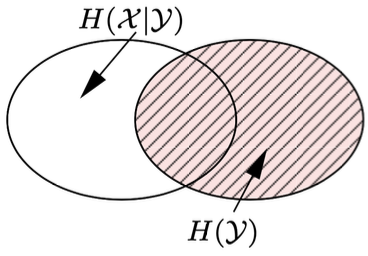
\includegraphics[scale = 0.7]{condentropy.png}
    \end{minipage}
    \hspace{0.2cm}
    \begin{minipage}{.5\textwidth}
        \centering
        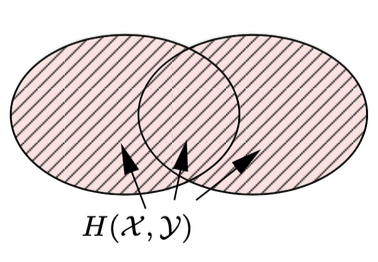
\includegraphics[scale = 0.7]{jointentropy.png}
    \end{minipage}
    \caption{Conditional entropy}
    \label{fig:condentropy}
\end{figure}

To implement this, the joint entropy function is applied to the joint probability distribution and the entropy function is applied to the sum on axis zero of the joint probability distribution to obtain $P(\mathcal{Y})$. 

\subsection*{Question 4 : Mutual Information}
The mutual information measures the dependence between a set of random variables. If the set of random variables is independent, the mutual information is equal to zero. The higher this measure, the higher the dependency between the random variables. \\

If $\mathcal{X}$ and $\mathcal{Y}$ are discrete random variables, $P\left(X_i \cap Y_j\right)$ is the probability of the random variable $\mathcal{X}$ to be $\mathcal{X}_i$ and in the same time the random variable $\mathcal{Y}$ to be $\mathcal{Y}_j$. Also, $P(\mathcal{X}_i)$ is the probability of the event $\mathcal{X}_i$ and $P(\mathcal{Y}_j)$ the probability of the event $\mathcal{Y}_j$. Then, the mutual information is defined as : 

$$I(\mathcal{X} ; \mathcal{Y})=+\sum_{i=1}^n \sum_{j=1}^m P\left(\mathcal{X}_i \cap \mathcal{Y}_j\right) \log \frac{P\left(\mathcal{X}_i \cap \mathcal{Y}_j\right)}{P\left(\mathcal{X}_i\right) P\left(\mathcal{Y}_j\right)}$$

In order to compute the mutual information with the probability distribution $P\left(\mathcal{X}_i \cap \mathcal{Y}_j\right)$, the formula needs to be rewritten as in slide 6 of the second course :

$$I(\mathcal{X} ; \mathcal{Y})=H(\mathcal{X})+H(\mathcal{Y})-H(\mathcal{X}, \mathcal{Y})$$

It can be proved graphically in the figure \ref{fig:mutualinfo} : 

\begin{figure}[h!]
    \begin{minipage}{.5\textwidth}
        \centering
        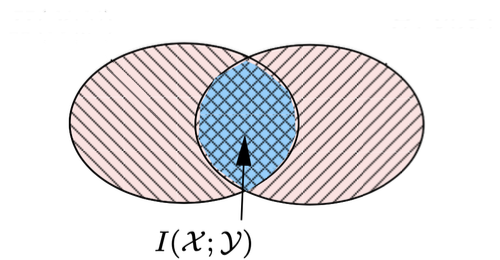
\includegraphics[scale = 0.7]{mutualinfo.png}
    \end{minipage}
    \hspace{0.2cm}
    \begin{minipage}{.5\textwidth}
        \centering
        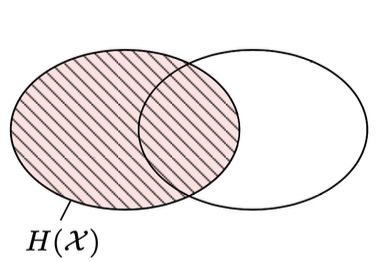
\includegraphics[scale = 0.7]{entropyx.png}
    \end{minipage}
\end{figure}
\begin{figure}[h!]
    \begin{minipage}{.5\textwidth}
        \centering
        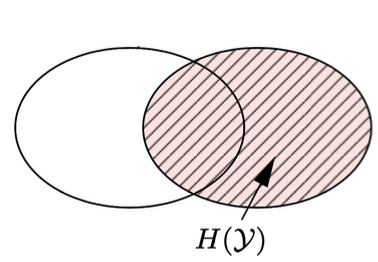
\includegraphics[scale = 0.7]{entropyy.png}
    \end{minipage}
    \hspace{0.2cm}
    \begin{minipage}{.5\textwidth}
        \centering
        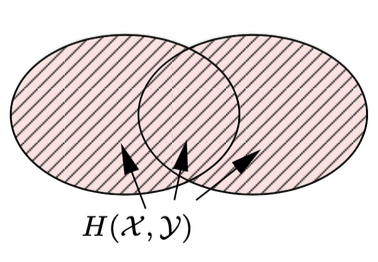
\includegraphics[scale = 0.7]{jointentropy.png}
    \end{minipage}
    \caption{Mutual Information}
    \label{fig:mutualinfo}
\end{figure}

To compute all the measures needed in the formula above, $P(\mathcal{X})$ and $P(\mathcal{Y})$ need to be defined. A sum is done on the joint probability matrix, on axis zero to obtain  $P(\mathcal{Y})$ and on axis one to obtain $P(\mathcal{X})$. Then, the entropy function is applied to these two vectors and the joint entropy function is applied to the joint probability distribution. 

\subsection*{Question 5 : Conditional joint entropy and conditional mutual information}

\subsubsection*{Conditional joint entropy}

If $\mathcal{X}$, $\mathcal{Y}$, $\mathcal{Z}$ are three random variables, the conditional joint entropy of $\mathcal{X}$, $\mathcal{Y}$ given $\mathcal{Z}$ is defined as : 

$$H(\mathcal{X}, \mathcal{Y} \mid \mathcal{Z})=H(\mathcal{X} \mid \mathcal{Z})+H(\mathcal{Y} \mid \mathcal{X}, \mathcal{Z})$$

It can be proved graphically in the figure \ref{fig:condjoint} : 

\begin{figure}[H]
    \centering
    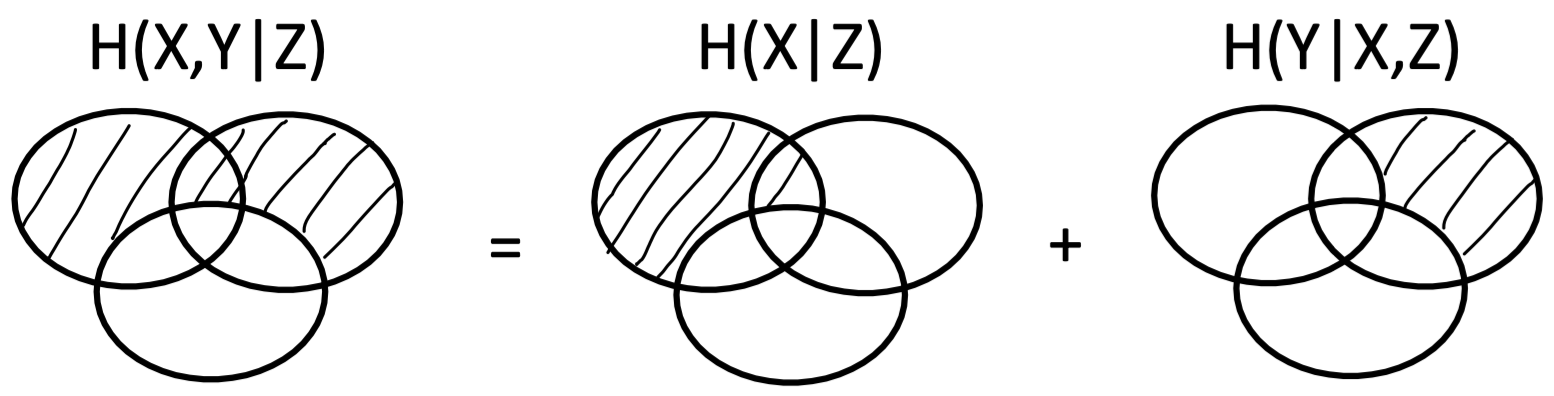
\includegraphics[scale = 0.28]{condjoint.png}
    \caption{Conditional joint entropy}
    \label{fig:condjoint}
\end{figure}

To implement this formula, the entropy function is used to compute $H(\mathcal{X} \mid \mathcal{Z})$. The conditional entropy $H(\mathcal{Y} \mid \mathcal{X}, \mathcal{Z})$ is computed thanks to the Bayes theorem : 

$$P(Y \mid X,Z) = \frac{P(\mathcal{X} \cap \mathcal{Y} \cap \mathcal{Z})}{P(\mathcal{X} \cap \mathcal{Z})}$$
 
\subsubsection*{Conditional mutual information}

If $\mathcal{X}$, $\mathcal{Y}$, $\mathcal{Z}$ are three random variables, the conditional mutual information of $\mathcal{X}$, $\mathcal{Y}$ given $\mathcal{Z}$ is defined as on slide 10 of the second course :  

$$ I(\mathcal{X} ; \mathcal{Y} \mid \mathcal{Z}) \triangleq H(\mathcal{X} \mid \mathcal{Z})-H(\mathcal{X} \mid \mathcal{Y}, \mathcal{Z})$$

To implement this formula, to compute $H(\mathcal{X} \mid \mathcal{Z})$, the conditional entropy function is applied on the joint probability distribution of $\mathcal{X}$ and $\mathcal{Z}$. $H(\mathcal{X} \mid \mathcal{Y}, \mathcal{Z})$ needs to be rewritten as : 

$$H(\mathcal{X} \mid \mathcal{Y}, \mathcal{Z})=-\sum_{i=1}^n \sum_{j=1}^m \sum_{k=1}^l(P(\mathcal{X}_i \cap \mathcal{Y}_j \cap \mathcal{Z}_k)) \log _2(P(\mathcal{X}_i \mid \mathcal{Y}_j, \mathcal{Z}_k))$$

where $P(\mathcal{X}_i \mid \mathcal{Y}_j, \mathcal{Z}_k)$ can be rewritten thanks to the Bayes rule as : 

$$P(\mathcal{X} \mid \mathcal{Y}, \mathcal{Z}) = \frac{P(\mathcal{X} \cap \mathcal{Y} \cap \mathcal{Z})}{P(\mathcal{Y} \cap \mathcal{Z})}$$

\newpage 

\section{Predicting the outcome of a football game}

\subsection*{Question 6 : Entropy and cardinality}

In the table \ref{tab:entropy}, the entropy and the cardinality of each variable can be found. 

\begin{table}[h!]
    \centering
    \small
    \setlength{\tabcolsep}{4pt}
    \begin{tabular}{|p{3cm}|p{2cm}|p{2cm}|}
        \hline 
        \textbf{Variable} & \textbf{Cardinality} & \textbf{Entropy}  \\
        \hline
        \textit{outcome} & 3 & 1.33488\\
        \hline
        \textit{previous\_outcome} & 3 & 1.483\\
        \hline
        \textit{day} & 7 & 2.80656\\
        \hline
        \textit{time} & 3 & 0.93252\\
        \hline
        \textit{month} & 12 & 3.58263\\
        \hline
        \textit{wind\_speed} & 3 & 1.58471\\
        \hline
        \textit{weather} & 4 & 1.76408\\
        \hline
        \textit{location} & 2 & 0.99994\\
        \hline
        \textit{capacity} & 4 & 1.53391\\
        \hline
        \textit{stadium\_state} & 2 & 0.63955\\
        \hline
        \textit{injury} & 2 & 0.99984\\
        \hline
        \textit{match\_type} & 2 & 0.9999\\
        \hline
        \textit{opponent\_strength} & 3 & 1.58435\\
        \hline
    \end{tabular}
    \caption{Cardinality and entropy of each variable}
    \label{tab:entropy}
\end{table}

Variables with a higher/lower cardinality typically have higher/lower entropy, which corresponds to higher/lower levels of uncertainty or randomness in the values of those variables. For instance, in contrast to the \textit{location} variable, the \textit{month} variable has a much higher entropy value.\\

If a variable's values are distributed evenly/not evenly for a given cardinality, the entropy may be higher/lower. For instance, with a cardinality of 2, the \textit{stadium\_state} variable has a lower entropy than the other variables with the same cardinality because the value \textit{dry} is much more prevalent than the value \textit{wet}. \\

Theoretically, if we look at the entropy's formula:

$$H(\mathcal{X}) \triangleq-\sum_{i=1}^n P\left(\mathcal{X}_i\right) \log_2 P\left(\mathcal{X}_i\right)$$

If a discrete random variable $\mathcal{X}$ has a larger/lower cardinality, then there are more/fewer potential values of $\mathcal{X}$ and the probabilities of these values are probably more dispersed/concentrated. As a result, the entropy value increases/decreases. \\

Moreover, the distribution of probabilities affects the entropy value.  If the probabilities are evenly distributed, because each value of  $\mathcal{X}$ is equally likely and there is more uncertainty, the entropy value will be larger. If they are not evenly distributed, because some values of $\mathcal{X}$ are more likely than others and there is less uncertainty, the entropy value will be lower.

\subsection*{Question 7 : Conditional entropy of \textit{outcome}}

\begin{table}[h!]
    \centering
    \small
    \setlength{\tabcolsep}{4pt}
    \begin{tabular}{|p{3cm}|p{4cm}|}
        \hline 
        \textbf{Variable} & \textbf{Conditional entropy}\\
        \hline
        \textit{previous\_outcome} & 1.18148\\
        \hline
        \textit{day} & 1.33349\\
        \hline
        \textit{time} & 1.3338\\
        \hline
        \textit{month} & 1.33036\\
        \hline
        \textit{wind\_speed} & 1.33473\\
        \hline
        \textit{weather} & 1.33384\\
        \hline
        \textit{location} & 1.33351\\
        \hline
        \textit{capacity} & 1.33202\\
        \hline
        \textit{stadium\_state} & 1.33432\\
        \hline
        \textit{injury} & 1.33024\\
        \hline
        \textit{match\_type} & 1.33483\\
        \hline
        \textit{opponent\_strength} & 0.93861\\
        \hline
    \end{tabular}
    \caption{Conditional entropy of \textit{outcome} given each of the other variables}
    \label{tab:q7_1}
\end{table}

\begin{table}[h!]
    \centering
    \small
    \setlength{\tabcolsep}{4pt}
    \begin{tabular}{|p{3cm}|p{2cm}|p{2cm}|}
        \hline 
        \textbf{Variable} & \textbf{Entropy}  \\
        \hline
        \textit{outcome} & 1.33488\\
        \hline
    \end{tabular}
    \caption{Entropy of \textit{outcome}}
    \label{tab:q7_2}
\end{table}

As it can be seen in the tables \ref{tab:q7_1} and \ref{tab:q7_2}, the conditional entropy of \textit{outcome} is very near to the entropy of \textit{outcome} when \textit{wind\_speed} is the conditioning variable. It shows that \textit{wind\_speed} has little impact on the uncertainty or randomness of \textit{outcome}. According to this, \textit{wind\_speed} is not a reliable predictor of \textit{outcome}.\\

The conditional entropy of \textit{outcome} is lower when \textit{previous\_outcome} is the conditioning variable. It shows that \textit{previous\_outcome} is a powerful predictor of \textit{outcome}. Thus, a performance's past behavior is a reliable predictor of its present behavior.

\newpage

\subsection*{Question 8 : Mutual information between \textit{month} and \textit{capacity}}

The table \ref{tab:q8} displays the mutual information between \textit{month} and \textit{capacity} as well as the mutual information between \textit{day} and \textit{time}. 

\begin{table}[h!]
    \centering
    \small
    \setlength{\tabcolsep}{4pt}
    \begin{tabular}{|p{4cm}|p{4cm}|}
        \hline 
        \textbf{Variables} & \textbf{Mutual information}\\
        \hline
        \textit{month and capacity} & 0.00607\\
        \hline
        \textit{day and time} & 0.50461\\
        \hline
    \end{tabular}
    \caption{Mutual information}
     \label{tab:q8}
\end{table}

With a mutual information of only 0.00607, it can be concluded that there is a small correlation between \textit{month} and \textit{capacity}. In other words, little knowledge about the value of one variable does not reveal much about the value of the other. This implies these factors are largely independent of one another, and they might not even need to be taken into account simultaneously when developing predictive models.\\

On the other hand, the mutual information between \textit{day} and \textit{time} is fairly high at 0.50461, showing a close association between these two variables. A large amount of information regarding the value of the other variable can be learned from knowing the value of one variable. This implies these variables are interconnected and might need to be taken into account together when developing predictive models.

\subsection*{Question 9 : Conditional entropy and mutual information of \textit{outcome}}

\begin{table}[h!]
    \centering
    \small
    \setlength{\tabcolsep}{4pt}
    \begin{tabular}{|p{3cm}|p{4cm}|p{4cm}|}
        \hline 
        \textbf{Variable} & \textbf{Conditional entropy} & \textbf{Mutual information}\\
        \hline
        \textit{previous\_outcome} & 1.18148 & 0.1534\\
        \hline
        \textit{day} & 1.33349 & 0.00139\\
        \hline
        \textit{time} & 1.3338 & 0.00108\\
        \hline
        \textit{month} & 1.33036 & 0.00452\\
        \hline
        \textit{wind\_speed} & 1.33473 & 0.00015\\
        \hline
        \textit{weather} & 1.33384 & 0.00104\\
        \hline
        \textit{location} & 1.33351 & 0.00137\\
        \hline
        \textit{capacity} & 1.33202 & 0.00286\\
        \hline
        \textit{stadium\_state} & 1.33432 & 0.00055\\
        \hline
        \textit{injury} & 1.33024 & 0.00464\\
        \hline
        \textit{match\_type} & 1.33483 & 0.00005\\
        \hline
        \textit{opponent\_strength} & 0.93861 & 0.39627\\
        \hline
    \end{tabular}
    \caption{Conditional entropy and mutual information of 
    \textit{outcome} given each of the other variables}
    \label{tab:q9}
\end{table}

As can be seen in table \ref{tab:q9}, according to the mutual information, \textit{opponent\_strength} has the highest value, coming in at 0.39627. Hence, if we could only invest in one variable, we would do it on \textit{opponent\_strength}.\\ 

Also, if the choice is based on conditional entropy, \textit{opponent\_strength} is the variable that implies the lowest conditional entropy of \textit{outcome} with 0.93861. As a result, if conditional entropy is used to make the decision, we would also select \textit{opponent\_strength}.

\newpage

\subsection*{Question 10 : Conditional mutual information of \textit{outcome}}
The table \ref{tab:q10} displays the mutual information between \textit{outcome} and each other variables given \textit{previous\_outcome}. 

\begin{table}[h!]
    \centering
    \small
    \setlength{\tabcolsep}{4pt}
    \begin{tabular}{|p{4cm}|p{4cm}|}
        \hline 
        \textbf{Variable} & \textbf{Mutual information}\\
        \hline
        \textit{day} & 0.00474\\
        \hline
        \textit{time} & 0.00347\\
        \hline
        \textit{month} & 0.01369\\
        \hline
        \textit{wind\_speed} & 0.00212\\
        \hline
        \textit{weather} & 0.00303\\
        \hline
        \textit{location} & 0.00213\\
        \hline
        \textit{capacity} & 0.00495\\
        \hline
        \textit{stadium\_state} & 0.00062\\
        \hline
        \textit{injury} & 0.009\\
        \hline
        \textit{match\_type} & 0.00051\\
        \hline
        \textit{opponent\_strength} & 0.24459\\
        \hline
    \end{tabular}
    \caption{Mutual Information between \textit{outcome} and each other variables given \textit{previous\_outcome}}
    \label{tab:q10}
\end{table}

The \textit{opponent\_strength} variable is still the best to invest in given the new information that the outcome of previous matches between the same opponent are now freely available. As it can be seen in the new data, while taking into consideration the outcome of previous matches, the mutual information between \textit{outcome} and \textit{opponent\_strength} reduces from 0.39627 to 0.24459 which shows that some of the knowledge provided by \textit{opponent\_strength} about \textit{outcome} is contained in \textit{previous\_outcome}. Moreover the amount of information provided by all the other variables increases when \textit{previous\_outcome}'s information is taken into consideration. But 0.24459 is still the highest. The \textit{opponent\_strength} variable is therefore still the most useful for forecasting the outcome of the game. 

\subsection*{Question 11 : Mutual information of \textit{location}}

\begin{table}[h!]
    \centering
    \small
    \setlength{\tabcolsep}{4pt}
    \begin{tabular}{|p{4cm}|p{4cm}|}
        \hline 
        \textbf{Variables} & \textbf{Mutual information}\\
        \hline
        \textit{stadium\_state and weather} & 0.0\\
        \hline
    \end{tabular}
    \caption{Mutual information when \textit{location} is home}
    \label{tab:q11}
\end{table}

As can be seen in the table \ref{tab:q11}, when the \textit{location} is home, the mutual information between \textit{stadium\_state} and \textit{weather} is equal to 0.0, indicating that the two variables are independent of one another.\\

It's conceivable that the home stadium has a unique microclimate unaffected by the weather outside. For instance, the stadium might be built in a protected place or have a roof over it to keep the weather out. Despite the fact they might be associated in other places, this thus results in the \textit{stadium\_state} variable being independent of the \textit{weather} variable.

\section{Playing with information theory-based strategy}

\subsection*{Question 12 : Entropy computation}

In this situation, all colors have the same probability to be on the board. The probability distribution for one slot is uniform and written as $P(X_i) = \frac{1}{6}$ for i $= 1,...,6$. Each slot is independent. Therefore, their entropy is the same. 

$$ H(X) = - log_2\left(\frac{1}{6}\right) = 2,59$$

The probability of the whole game for each color is the same. The game can accept $6^4$ combinations. The probability distribution for the whole game is uniform and is written as $P(X_i) = \frac{1}{6} * \frac{1}{6} * \frac{1}{6} * \frac{1}{6} = (\frac{1}{6})^4$ with i = 1, ..., 6  because the whole game is made of four slots. The entropy is then : 

$$ H(X) = - log_2\left(\left(\frac{1}{6}\right)^4\right) = 10,34$$

The two entropies are linked by the factor 4, due to the four slots present in the whole game. 

\subsection*{Question 13 : First Guess}

Firstly, the slot for which the guess is right, its entropy is equal to zero since the probability for this slot for this color is equal to one and the others are zero. Secondly, two cases are possible. The first case is if the correct color is the red or the yellow slot. If it is the case, each cell has now a probability of $\frac{1}{4}$ for each color. For instance, if the first slot is the correct one, the blue slots and the green slot can be neither green or blue. Four colors are left to complete the slots. The entropy for the wrong slots is then : 

$$H(\text{Each slot left}) = - log_2\left(\frac{1}{4}\right) = 2$$. 

And the entropy for the whole board is :

$$H(\text{Whole board}) = 3 * H(\text{Each slot left}) = 6$$

The second case is if the correct color is one of the blue slot. Then, the red, green and the other slot can neither be blue, green or red. The slots have only three colors left to be. Each cell has now a probability of $\frac{1}{3}$ for each color. In this case, the entropy is 

$$H(X_i) = - log_2\left(\frac{1}{3}\right) = 1,58$$

And the entropy for the whole board is : 

$$H(\text{Whole board}) = 3 * H(\text{Each slot left}) = 4,74$$

Now, the entropy needs to be generalized for all possibilities. The expectation of the two entropies will give the generalized value for the entropy. 

$$H(\text{Whole board}) = \frac{6 + 4,74}{2} = 5,37$$

The information obtained is H$_{stage0}$ - H$_{stage1}$ = $10,34 - 5,37 = 4,97$, meaning the information can be represented in 5 bits.

\subsection*{Question 14 : First guess bis}

For this question, a lot of cases are possible. Some of the cases have the same entropy. First, as before, the slots that have been correctly guessed have always an entropy equal to zero. \\

First case, the slot one or three are the correct ones and one of the blue slot is the incorrect one. This situation happens four times. The table \ref{tab:case1} shows the probability distribution of one of this situation :

\begin{table}[h!]
\centering
\begin{tabular}{|c|c|c|c|c|}
        \hline
        Colours / Slot number & 1 & 2 & 3 & 4 \\ 
        \hline
        1 & 1 & 1/4 & 0 & 1/4 \\
        \hline
        2 & 0 & 0 & 1 & 1/4 \\
        \hline
        3 & 0 & 1/4 & 0 & 1/4 \\
        \hline
        4 & 0 & 0 & 0 & 0 \\
        \hline
        5 & 0 & 1/4 & 0 & 1/4 \\
        \hline
        6 & 0 & 1/4 & 0 & 1/4\\
        \hline
        Entropy & 0 & 2 & 0 & 2\\
        \hline
   
\end{tabular}
 \caption{Slot 1 is correct and slot 2 is incorrect}
 \label{tab:case1}
\end{table}


Thus, in these cases the total entropy is equal to 4. \\

Second case, the slot one or three are the correct or the incorrect slots. This case happens two times. The table \ref{tab:case2} shows the probability distribution of one of this situation.  

\begin{table}[h!]
\centering
\begin{tabular}{|c|c|c|c|c|}
        \hline
        Colours / Slot number & 1 & 2 & 3 & 4 \\ 
        \hline
        1 & 1 & 1/8 & 1/4 & 1/8\\
        \hline
        2 & 0 & 0 & 0 & 0\\
        \hline
        3 & 0 & 1/8 & 1/4 & 1/8 \\
        \hline
        4 & 0 & 1/2 & 0 & 1/2 \\
        \hline
        5 & 0 & 1/8 & 1/4 & 1/8 \\
        \hline
        6 & 0 & 1/8 & 1/4 & 1/8 \\
        \hline
        Entropy & 0 & 2 & 2 & 2 \\
        \hline     
\end{tabular}
\caption{Slot 1 is correct and slot 3 is incorrect}
\label{tab:case2}
\end{table}

Thus, in these cases the total entropy is equal to 6. \\

Third case, one of the blue slot is the correct one and the slots 1 or 3 is the incorrect one. This situation happens four times. The table \ref{tab:case3} shows the probability distribution of one of this situation : 

\begin{table}[h!]
\centering
\begin{tabular}{|c|c|c|c|c|}
        \hline
        Colours / Slot number & 1 & 2 & 3 & 4 \\ 
        \hline
        1 & 0 & 0 & 1/2 & 1/2 \\
        \hline
        2 & 0 & 1 & 0 & 0\\
        \hline
        3 & 1/3 & 0 & 1/6 & 1/6\\
        \hline
        4 & 0 & 0 & 0 & 0 \\
        \hline
        5 & 1/3 & 0 & 1/6 & 1/6\\
        \hline
        6 & 1/3 & 0 & 1/6 & 1/6 \\
        \hline
        Entropy & 1,58 & 0 & 1,79 & 1,79\\
        \hline
\end{tabular}
\caption{Slot 2 is correct and slot 1 is incorrect}
\label{tab:case3}
\end{table}

Thus, in these cases the total entropy is equal to 5,16. \\

Last case, the blue slots are the correct and the incorrect one. This situation happens in two cases. The table \ref{tab:case4} represents the probability distribution of one of this situation : 

\begin{table}[h!]
\centering
\begin{tabular}{|c|c|c|c|c|}
        \hline
        Colours / Slot number & 1 & 2 & 3 & 4 \\ 
        \hline
        1 & 0 & 0 & 0 & 0 \\
        \hline
        2 & 1/2 & 1 & 1/2 & 0\\
        \hline
        3 & 1/6 & 0 & 1/6 & 1/3\\
        \hline
        4 & 0 & 0 & 0 & 0 \\
        \hline
        5 & 1/6 & 0 & 1/6 & 1/3\\
        \hline
        6 & 1/6 & 0 & 1/6 & 1/3 \\
        \hline
        Entropy & 1,79 & 0 & 1,79 & 1,58\\
        \hline
\end{tabular}
\caption{Slot 2 is correct and slot 4 is incorrect}
\label{tab:case4}
\end{table}

Thus, in these cases the total entropy is equal to 5,16. \\

The whole entropy is the sum of each slot's entropy. All of these cases need to be generalized to one unique entropy. The expectation of these cases will give the generalized entropy :

$$H(\text{Whole board}) = \frac{4*4 + 2*6 + 6*5,16}{12} = 4,91$$

The information obtained is H$_{stage0}$ - H$_{stage1}$ = $10,34 - 4,91 = 5,43$, meaning the information can be represented in 5 bits.

\subsection*{Question 15 : Maximum entropy}

For one slot, with $\mathcal{C}$ as the number of possible colors, the formula would become : 

$$ H(\mathcal{X}_i) = -\log_2 \left(\frac{1}{\mathcal{C}}\right)$$
For the whole board, with $\mathcal{S}$ as the number of slot on the board, the formula would become : 

$$ H(\text{Whole board}) = \mathcal{S}*H(\mathcal{X}_i) = -\log_2 \left(\frac{1}{\mathcal{C}^{\mathcal{S}}}\right)$$

The log in base 2 is larger in absolute value for smaller values of probability. Thus, the higher the color number and the higher the slot number, the higher the entropy is. 

\subsection*{Question 16 : Optimized guessing }

In order to do the best guess at each round, we need to maximize the entropy of the guess colour code. It will maximize the amount of information given by the colour. \\

One method to do that is to first put four pawns of the same colour (whatever the colour). By doing this, the information we collect is if the colour we first choose is present on the board one or several times. \\

Secondly, if this colour is correct or incorrect, we keep one or several pawn of this colour (we will slide it at each step to know its exact position). Then, we fill the empty slots with another colour (all the same). It allows to see if the second color is on the board. We continue this strategy by adding another colour till the end to know all the colours that are present. With this technique, the entropy is maximized at each step. 
\newpage 

For instance, if the code to guess is 1 7 3 6 and our first guess is 2 2 2 2. The probability distribution looks like this : 

\begin{table}[h!]
\centering
\begin{tabular}{|c|c|c|c|c|}
        \hline
        Colours / Slot number & 1 & 2 & 3 & 4 \\ 
        \hline
        1 & 1/5 & 1/5 & 1/5 & 1/5 \\
        \hline
        2 & 0 & 0 & 0 & 0\\
        \hline
        3 & 1/5 & 1/5 & 1/5 & 1/5\\
        \hline
        4 & 1/5 & 1/5 & 1/5 & 1/5 \\
        \hline
        5 & 1/5 & 1/5 & 1/5 & 1/5\\
        \hline
        6 & 1/5 & 1/5 & 1/5 & 1/5 \\
        \hline
        Entropy & 2,32 & 2,32 & 2,32 & 2,32\\
        \hline
\end{tabular}
\end{table}

The total entropy is then 9,28 which is pretty high. We know that 2 is not on the board. Then, if we do a second guess as 3 3 3 3, we obtain the followed result : 

\begin{table}[h!]
\centering
\begin{tabular}{|c|c|c|c|c|}
        \hline
        Colours / Slot number & 1 & 2 & 3 & 4 \\ 
        \hline
        1 & 1/4 & 1/4 & 0 & 1/4 \\
        \hline
        2 & 0 & 0 & 0 & 0\\
        \hline
        3 & 0 & 1/4 & 1 & 1/4\\
        \hline
        4 & 1/4 & 1/4 & 0 & 1/4 \\
        \hline
        5 & 1/4 & 1/4 & 0 & 1/4\\
        \hline
        6 & 1/4 & 1/4 & 0 & 1/4 \\
        \hline
        Entropy & 2 & 2 & 2 & 2\\
        \hline
\end{tabular}
\end{table}
The total entropy at this step is then equal to 6 and still gives a lot of information for the next guess. If we continue this strategy, we will find the combination in a minimal of guesses. 

\end{document}
